% Icon of Saint Andrew the First-Called: no title, centred, between a top rule
% carrying a thistle and a plain bottom rule. The emblem is Scotland's, whose
% patron he is. Rules, thistle and icon are one picture, so they need no overlay
% pass to line up. No rule runs down either side.
\thispagestyle{empty}
\vspace*{\fill}
\begin{center}
\begin{tikzpicture}
  \node[inner sep=0pt] (icon) {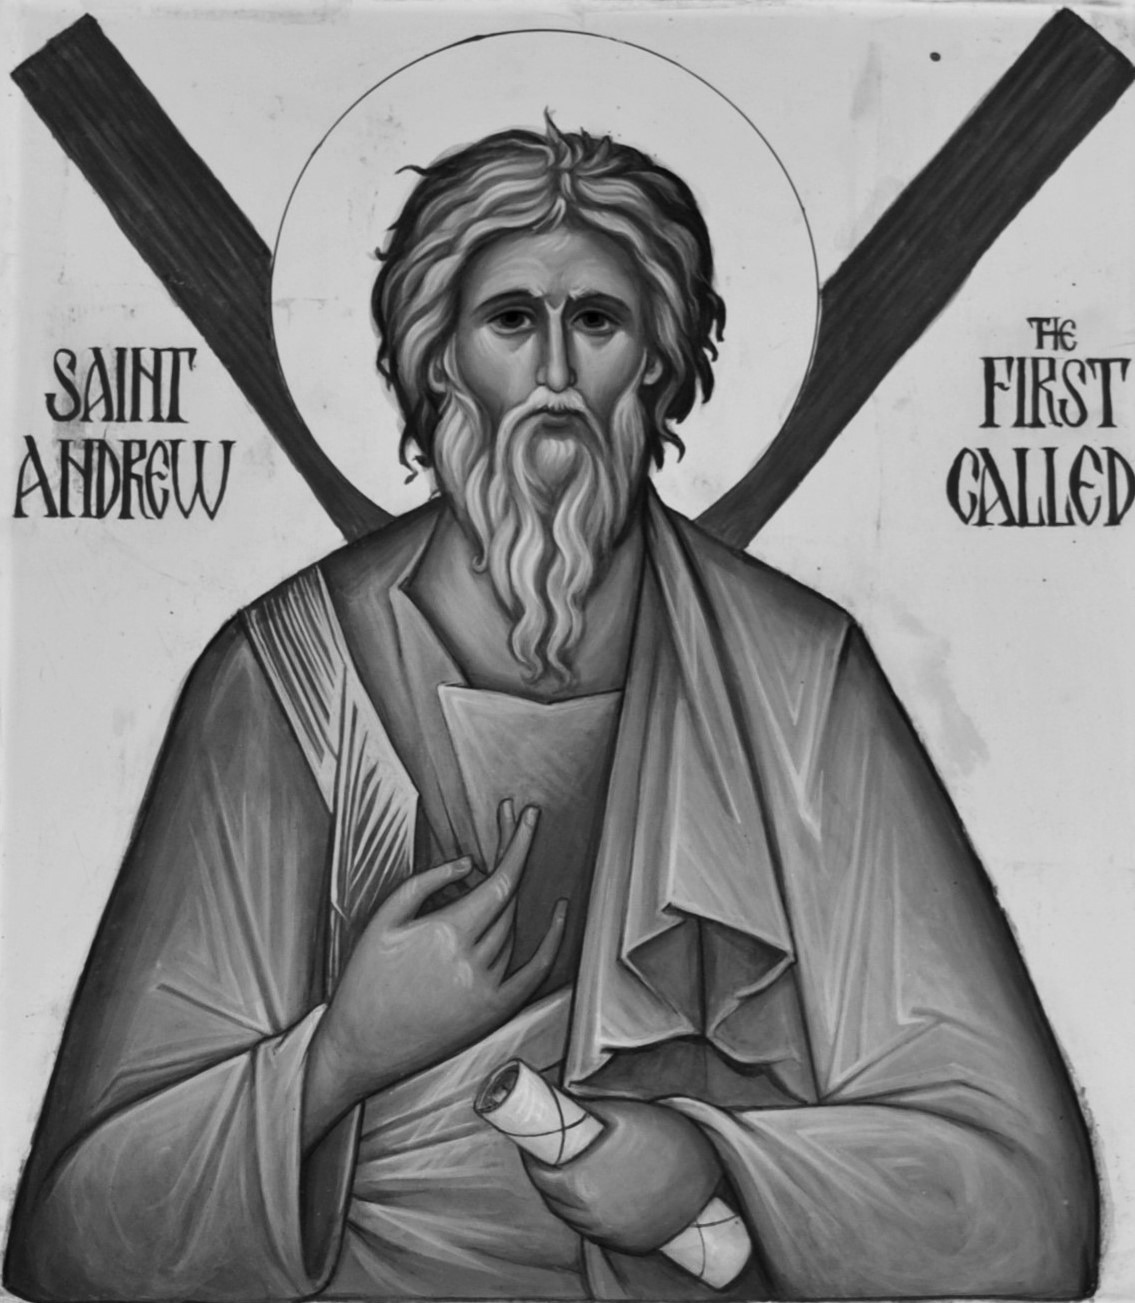
\includegraphics[width=68mm]{assets/icon.jpg}};

  \draw[line width=0.5pt] ([shift={(-4mm,4mm)}]icon.north west)
    -- ([shift={(4mm,4mm)}]icon.north east);
  \draw[line width=0.5pt] ([shift={(-4mm,-4mm)}]icon.south west)
    -- ([shift={(4mm,-4mm)}]icon.south east);

  \coordinate (ornament) at ([shift={(0,4mm)}]icon.north);
  \plumeornament{ornament}
\end{tikzpicture}
\end{center}
\vspace*{\fill}
\newpage
